%%%%%%%%%%%%%%%%%%%%%%%%%%%%%%%%%%%%%%%%%
% Lachaise Assignment
% LaTeX Template
% Version 1.0 (26/6/2018)
%
% This template originates from:
% http://www.LaTeXTemplates.com
%
% Authors:
% Marion Lachaise & François Févotte
% Vel (vel@LaTeXTemplates.com)
%
% License:
% CC BY-NC-SA 3.0 (http://creativecommons.org/licenses/by-nc-sa/3.0/)
% 
%%%%%%%%%%%%%%%%%%%%%%%%%%%%%%%%%%%%%%%%%

%----------------------------------------------------------------------------------------
%	PACKAGES AND OTHER DOCUMENT CONFIGURATIONS
%----------------------------------------------------------------------------------------

\documentclass{article}

\usepackage[utf8]{vietnam}
\usepackage{listings}
\usepackage{xcolor}
\usepackage{graphicx} % Required for the inclusion of images
\usepackage{natbib} % Required to change bibliography style to APA
\usepackage{amsmath} % Required for some math elements 
\usepackage{wrapfig}
\definecolor{codegreen}{rgb}{0,0.6,0}
\definecolor{codegray}{rgb}{0.5,0.5,0.5}
\definecolor{codepurple}{rgb}{0.58,0,0.82}
\definecolor{backcolour}{rgb}{0.95,0.95,0.92}

\lstdefinestyle{mystyle}{
    backgroundcolor=\color{backcolour},   
    commentstyle=\color{codegreen},
    keywordstyle=\color{magenta},
    numberstyle=\tiny\color{codegray},
    stringstyle=\color{codepurple},
    basicstyle=\ttfamily\footnotesize,
    breakatwhitespace=false,         
    breaklines=true,                 
    captionpos=b,                    
    keepspaces=true,                 
    numbers=left,                    
    numbersep=5pt,                  
    showspaces=false,                
    showstringspaces=false,
    showtabs=false,                  
    tabsize=2
}


\lstset{style=mystyle}


%%%%%%%%%%%%%%%%%%%%%%%%%%%%%%%%%%%%%%%%%
% Lachaise Assignment
% Structure Specification File
% Version 1.0 (26/6/2018)
%
% This template originates from:
% http://www.LaTeXTemplates.com
%
% Authors:
% Marion Lachaise & François Févotte
% Vel (vel@LaTeXTemplates.com)
%
% License:
% CC BY-NC-SA 3.0 (http://creativecommons.org/licenses/by-nc-sa/3.0/)
% 
%%%%%%%%%%%%%%%%%%%%%%%%%%%%%%%%%%%%%%%%%

%----------------------------------------------------------------------------------------
%	PACKAGES AND OTHER DOCUMENT CONFIGURATIONS
%----------------------------------------------------------------------------------------

\usepackage{amsmath,amsfonts,amssymb} % Math packages

\usepackage{enumerate} % Custom item numbers for enumerations

\usepackage[ruled]{algorithm2e} % Algorithms

\usepackage[framemethod=tikz]{mdframed} % Allows defining custom boxed/framed environments

\usepackage{listings} % File listings, with syntax highlighting
\lstset{
	basicstyle=\ttfamily, % Typeset listings in monospace font
}

%----------------------------------------------------------------------------------------
%	DOCUMENT MARGINS
%----------------------------------------------------------------------------------------

\usepackage{geometry} % Required for adjusting page dimensions and margins

\geometry{
	paper=a4paper, % Paper size, change to letterpaper for US letter size
	top=2.5cm, % Top margin
	bottom=3cm, % Bottom margin
	left=2.5cm, % Left margin
	right=2.5cm, % Right margin
	headheight=14pt, % Header height
	footskip=1.5cm, % Space from the bottom margin to the baseline of the footer
	headsep=1.2cm, % Space from the top margin to the baseline of the header
	%showframe, % Uncomment to show how the type block is set on the page
}

%----------------------------------------------------------------------------------------
%	FONTS
%----------------------------------------------------------------------------------------

%\usepackage[utf8]{inputenc} % Required for inputting international characters

\usepackage[utf8]{vietnam}



%----------------------------------------------------------------------------------------
%	COMMAND LINE ENVIRONMENT
%----------------------------------------------------------------------------------------

% Usage:
% \begin{commandline}
%	\begin{verbatim}
%		$ ls
%		
%		Applications	Desktop	...
%	\end{verbatim}
% \end{commandline}

\mdfdefinestyle{commandline}{
	leftmargin=10pt,
	rightmargin=10pt,
	innerleftmargin=15pt,
	middlelinecolor=black!50!white,
	middlelinewidth=2pt,
	frametitlerule=false,
	backgroundcolor=black!5!white,
	frametitle={Command Line},
	frametitlefont={\normalfont\sffamily\color{white}\hspace{-1em}},
	frametitlebackgroundcolor=black!50!white,
	nobreak,
}

% Define a custom environment for command-line snapshots
\newenvironment{commandline}{
	\medskip
	\begin{mdframed}[style=commandline]
}{
	\end{mdframed}
	\medskip
}

%----------------------------------------------------------------------------------------
%	FILE CONTENTS ENVIRONMENT
%----------------------------------------------------------------------------------------

% Usage:
% \begin{file}[optional filename, defaults to "File"]
%	File contents, for example, with a listings environment
% \end{file}

\mdfdefinestyle{file}{
	innertopmargin=1.6\baselineskip,
	innerbottommargin=0.8\baselineskip,
	topline=false, bottomline=false,
	leftline=false, rightline=false,
	leftmargin=2cm,
	rightmargin=2cm,
	singleextra={%
		\draw[fill=black!10!white](P)++(0,-1.2em)rectangle(P-|O);
		\node[anchor=north west]
		at(P-|O){\ttfamily\mdfilename};
		%
		\def\l{3em}
		\draw(O-|P)++(-\l,0)--++(\l,\l)--(P)--(P-|O)--(O)--cycle;
		\draw(O-|P)++(-\l,0)--++(0,\l)--++(\l,0);
	},
	nobreak,
}

% Define a custom environment for file contents
\newenvironment{file}[1][File]{ % Set the default filename to "File"
	\medskip
	\newcommand{\mdfilename}{#1}
	\begin{mdframed}[style=file]
}{
	\end{mdframed}
	\medskip
}

%----------------------------------------------------------------------------------------
%	NUMBERED QUESTIONS ENVIRONMENT
%----------------------------------------------------------------------------------------

% Usage:
% \begin{question}[optional title]
%	Question contents
% \end{question}

\mdfdefinestyle{question}{
	innertopmargin=1.2\baselineskip,
	innerbottommargin=0.8\baselineskip,
	roundcorner=5pt,
	nobreak,
	singleextra={%
		\draw(P-|O)node[xshift=1em,anchor=west,fill=white,draw,rounded corners=5pt]{%
		Question \theQuestion\questionTitle};
	},
}

\newcounter{Question} % Stores the current question number that gets iterated with each new question

% Define a custom environment for numbered questions
\newenvironment{question}[1][\unskip]{
	\bigskip
	\stepcounter{Question}
	\newcommand{\questionTitle}{~#1}
	\begin{mdframed}[style=question]
}{
	\end{mdframed}
	\medskip
}

%----------------------------------------------------------------------------------------
%	WARNING TEXT ENVIRONMENT
%----------------------------------------------------------------------------------------

% Usage:
% \begin{warn}[optional title, defaults to "Warning:"]
%	Contents
% \end{warn}

\mdfdefinestyle{warning}{
	topline=false, bottomline=false,
	leftline=false, rightline=false,
	nobreak,
	singleextra={%
		\draw(P-|O)++(-0.5em,0)node(tmp1){};
		\draw(P-|O)++(0.5em,0)node(tmp2){};
		\fill[black,rotate around={45:(P-|O)}](tmp1)rectangle(tmp2);
		\node at(P-|O){\color{white}\scriptsize\bf !};
		\draw[very thick](P-|O)++(0,-1em)--(O);%--(O-|P);
	}
}

% Define a custom environment for warning text
\newenvironment{warn}[1][Warning:]{ % Set the default warning to "Warning:"
	\medskip
	\begin{mdframed}[style=warning]
		\noindent{\textbf{#1}}
}{
	\end{mdframed}
}

%----------------------------------------------------------------------------------------
%	INFORMATION ENVIRONMENT
%----------------------------------------------------------------------------------------

% Usage:
% \begin{info}[optional title, defaults to "Info:"]
% 	contents
% 	\end{info}

\mdfdefinestyle{info}{%
	topline=false, bottomline=false,
	leftline=false, rightline=false,
	nobreak,
	singleextra={%
		\fill[black](P-|O)circle[radius=0.4em];
		\node at(P-|O){\color{white}\scriptsize\bf i};
		\draw[very thick](P-|O)++(0,-0.8em)--(O);%--(O-|P);
	}
}

% Define a custom environment for information
\newenvironment{info}[1][Info:]{ % Set the default title to "Info:"
	\medskip
	\begin{mdframed}[style=info]
		\noindent{\textbf{#1}}
}{
	\end{mdframed}
}
 % Include the file specifying the document structure and custom commands

%----------------------------------------------------------------------------------------
%	ASSIGNMENT INFORMATION
%----------------------------------------------------------------------------------------

\title{Web Technologies: Nhóm Web  \#1} % Title of the assignment

\author{Bùi Quang Đức: 20173023 \\ Vũ Đức Hòa: 20173121 \\ Trần Đình Đức: 20173028 \\ Trần Duy Hải: 20173091 \\ Giảng viên: TS. Đào Thành Chung}} % Author name and email address

\date{Hanoi University of Science and Technology --- \today} % University, school and/or department name(s) and a date

%----------------------------------------------------------------------------------------

\begin{document}

\maketitle % Print the title

%----------------------------------------------------------------------------------------
%	INTRODUCTION
%----------------------------------------------------------------------------------------

\section*{Phân công công việc trong nhóm Web}

\begin{itemize}
\item Thiết kế UI: Bùi Quang Đức, Trần Duy Hải
\item Lập trình Backend PHP: Trần Đình Đức, Vũ Đức Hòa
\item Thiết kế Database, thu tập dữ liệu: Vũ Đức Hòa
\item Tạo tệp tin trình bày (Slide): Vũ Đức Hòa
\item Tạo tệp tin báo cáo: Bùi Quang Đức
\end{itemize}

%------------------------------------------------

\section*{Tổng quan bài tập lớn} % Unnumbered section

Website chia sẻ kiến thức và kinh nghiệm lập trình. Với mong muốn chia sẻ những điều thuộc lĩnh vực công nghệ thông tin cho mọi người không phân biệt lứa tuổi.

Bên cạnh việc chia sẻ, nhận những phản hồi từ người dùng, website chia sẻ kiến thức và kinh nghiệm lập trình cho phép chúng ta tương tác giữa người dùng và quản trị thông qua những comment cuốn hút.

\begin{info}[Lưu ý:] % Information block
Website chia sẻ kiến thức lập trình nên có thể không phù hợp với đối tượng không am hiểu hay biết vể kiến thức công nghệ thông tin, vì thế nếu tham gia vào mạng xã hội của chúng tôi mà đọc không hiểu gì vui lòng đừng thêm những comment gây thù ghét.
\end{info}

%----------------------------------------------------------------------------------------
%	PROBLEM 1
%----------------------------------------------------------------------------------------

\section*{Các chức năng chính của website} % Numbered section

Website chia sẻ kiến thức và kinh nghiệm lập trình cũng như hiểu biết về công nghệ thông tin gồm một số chức năng thông dụng và rất nhiều chức năng nâng cao sẽ có trong tương lai (sau deadline :3)

\begin{itemize}
\item Đăng nhập, đăng ký
\item Xem bài viết
\item Tìm kiếm bài viết theo từ khóa, danh mục
\item Quản lý bài viết, chủ đề, người dùng
\end{itemize}
%------------------------------------------------
\newpage
\section*{Cấu trúc của chương trình}

\begin{figure}[h]
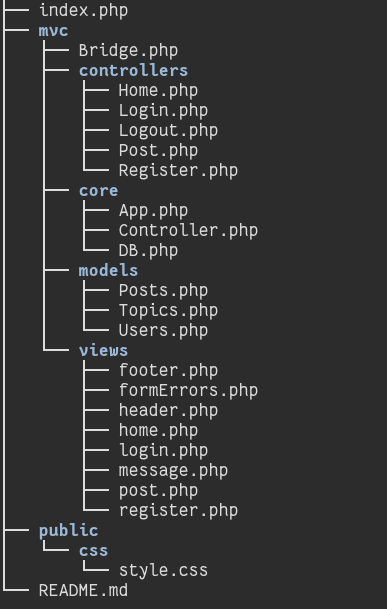
\includegraphics[width=.5\linewidth]{image/site.png}
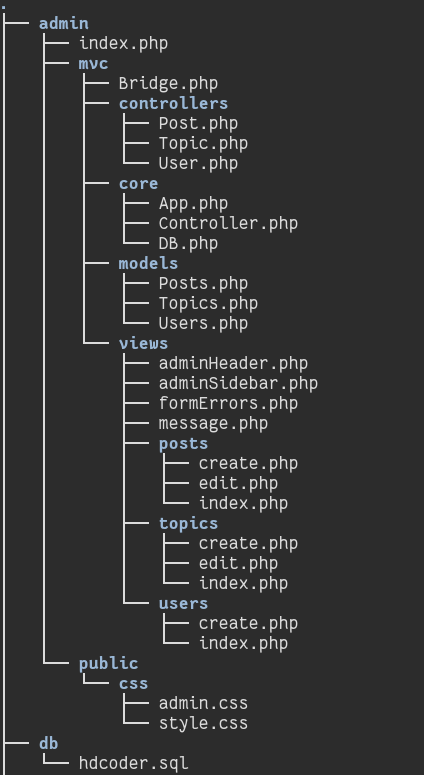
\includegraphics[width=.5\linewidth]{image/user.png}
\end{figure}

\newpage

\section*{Một số công nghệ đã sử dụng}

\begin{itemize}
\item Giao diện: HTML5, CSS3, Javascript
\item Server: PHP theo mô hình MVC
\item Cơ sở dữ liệu: MySQL
\item Sử dụng hàm băm cho mật khẩu khi tương tác với cơ sở dữ liệu (hàm password\_hash()) 
\item Sử dụng prepared statement cho các câu truy vấn nhằm tránh vấn đề bảo mật SQL Injection (trong tương lai nhóm sẽ có gắn thêm 1 anti-csrf token)
\end{itemize}

\section*{Hướng phát triển trong tương lai}

\begin{itemize}
\item Cho phép người dùng đăng bài viết
\item Tạo hệ thống kiểm duyệt tự động
\item Chức năng bình luận, rating cho người dùng
\item Sử dụng AJAX Live Search

\begin{lstlisting}[language=html, caption=The HTML Page]

<html>
<head>
<script>
function showResult(str) {
  if (str.length==0) {
    document.getElementById("livesearch").innerHTML="";
    document.getElementById("livesearch").style.border="0px";
    return;
  }
  var xmlhttp=new XMLHttpRequest();
  xmlhttp.onreadystatechange=function() {
    if (this.readyState==4 && this.status==200) {
      document.getElementById("livesearch").innerHTML=this.responseText;
      document.getElementById("livesearch").style.border="1px solid #A5ACB2";
    }
  }
  xmlhttp.open("GET","livesearch.php?q="+str,true);
  xmlhttp.send();
}
</script>
</head>
<body>

<form>
<input type="text" size="30" onkeyup="showResult(this.value)">
<div id="livesearch"></div>
</form>

</body>
</html>

\end{lstlisting}

\begin{lstlisting}[language=php, caption=The PHP File]

<?php
$xmlDoc=new DOMDocument();
$xmlDoc->load("links.xml");

$x=$xmlDoc->getElementsByTagName('link');

//get the q parameter from URL
$q=$_GET["q"];

//lookup all links from the xml file if length of q>0
if (strlen($q)>0) {
  $hint="";
  for($i=0; $i<($x->length); $i++) {
    $y=$x->item($i)->getElementsByTagName('title');
    $z=$x->item($i)->getElementsByTagName('url');
    if ($y->item(0)->nodeType==1) {
      //find a link matching the search text
      if (stristr($y->item(0)->childNodes->item(0)->nodeValue,$q)) {
        if ($hint=="") {
          $hint="<a href='" .
          $z->item(0)->childNodes->item(0)->nodeValue .
          "' target='_blank'>" .
          $y->item(0)->childNodes->item(0)->nodeValue . "</a>";
        } else {
          $hint=$hint . "<br /><a href='" .
          $z->item(0)->childNodes->item(0)->nodeValue .
          "' target='_blank'>" .
          $y->item(0)->childNodes->item(0)->nodeValue . "</a>";
        }
      }
    }
  }
}

// Set output to "no suggestion" if no hint was found
// or to the correct values
if ($hint=="") {
  $response="no suggestion";
} else {
  $response=$hint;
}

//output the response
echo $response;
?>
\end{lstlisting}

\end{itemize}


% Warning text, with a custom title
\begin{warn}[Kết luận:]
Nhờ học phần Công nghệ Web gắn với bài tập lớn, nhóm đã có thêm vô vàn kiến thức về lập trình web, cũng như hiểu hơn về những mô hình website khác, nắm bắt được rất nhiều những thông tin về thế giới công nghệ thông tin đầy màu sắc.
Cảm ơn thầy (hoặc các độc giả khác) đã đọc bản thu hoạch bài tập lớn của nhóm.
Nhóm Web xin trân trọng cảm ơn!
\end{warn}

%----------------------------------------------------------------------------------------

\end{document}
